\documentclass[a4paper,11pt]{report}

\usepackage{fullpage}

\usepackage{amsmath}
\usepackage{bussproofs}
\usepackage{mathpartir}
\usepackage{prooftrees}
\usepackage{color}

% for finite state automata
\usepackage{tikz}
\usetikzlibrary{automata,positioning}

\author{Sylvain Julmy}
\date{\today}

\setlength{\parindent}{0pt}

\begin{document}

\begin{center}
  \Large{
    Operating Systems\\
    Spring 2018
  }
  
  \noindent\makebox[\linewidth]{\rule{\linewidth}{0.4pt}}
  S01
  \noindent\makebox[\linewidth]{\rule{\linewidth}{0.4pt}}

  \begin{flushleft}
    Professor : Philippe Cudré-Mauroux

    Assistant : Ines Arous
  \end{flushleft}
  
  \noindent\makebox[\linewidth]{\rule{\linewidth}{0.4pt}}

  Submitted by Sylvain Julmy
  
  \noindent\makebox[\linewidth]{\rule{\textwidth}{1pt}}
\end{center}

\section*{Exercice 2}

\subsection*{a)}

In kernel mode, the executing code has a complete access to the hardware. There
is no restriction about it. The code can do almost anything from executing any
CPU instruction or accessing any memory address.

In user mode, the executing code has to use system call in order to access
low-level functionnality like memory allocation. The executing code memory is
allocated by the system and the code don't have any access to the memory of the
other running code.

Having two separate mode is usefull in designing an operating system for the
following reason :
\begin{itemize}
\item The critical code which are purely system related are running in kernel
  mode for efficiency. Those code have to be sure and idealy certified and
  verified.
\item Any non-system related code run in user mode, because any failure of the
  code would be recoverable due to the memory management by the system.
\end{itemize}

\subsection*{b)}

Only reading the time-of-day clock should be allowed in user mode as well as in
kernel mode. All other instructions should be only allowed in kernel mode for
security.

\subsection*{c)}

\paragraph{Advantages :}
\begin{itemize}
\item Increase the hardware utilisation.
\item Decrease capital and operating cost.
\item Run program in a VM which maybe canno't run on the physical one due to
  operating system compatibility.
\item We can save the state of a VM.
\item VM are isolated from the host machine. In case of malware, the host is safe.
\end{itemize}

\paragraph{Disadvantage :}
\begin{itemize}
\item The host has to be accessible in order for all the VM to be accessible.
\item The VM don't have a direct access to the hardware.
\item Increased memory and processor usage as part of overhead introduced by the VM.
\item When multiple virtual machines are simultaneously running on a host
  computer, each virtual machine may introduce an unstable performance, which
  depends on the workload on the system by other running virtual machines.
\end{itemize}

\section*{Exercice 3}

\subsection*{a)}

Using the command \verb|htop|, we can visualize the number of CPU of the
computer and the memory usage of the system.

\begin{figure}[ht]
  \centering
  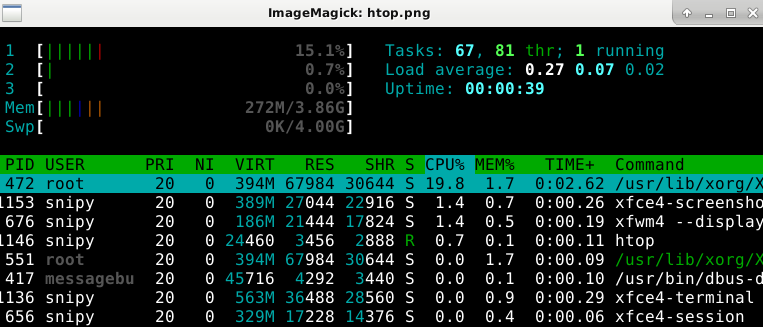
\includegraphics[width=0.9\textwidth]{img/htop}
\end{figure}

The command simply show so information about the current system state and all
the active process.

\paragraph{Number of CPU :} $3$

\paragraph{How much memory :} $3.86G$

\paragraph{Fraction of the memory used :} $272M / 3.86G$

\newpage

\subsection*{b)}

In order to construct the complete tree of the processes, we can use \verb|htop|
too. The command has an option which construct the tree for us :

\begin{figure}[h]
  \centering
  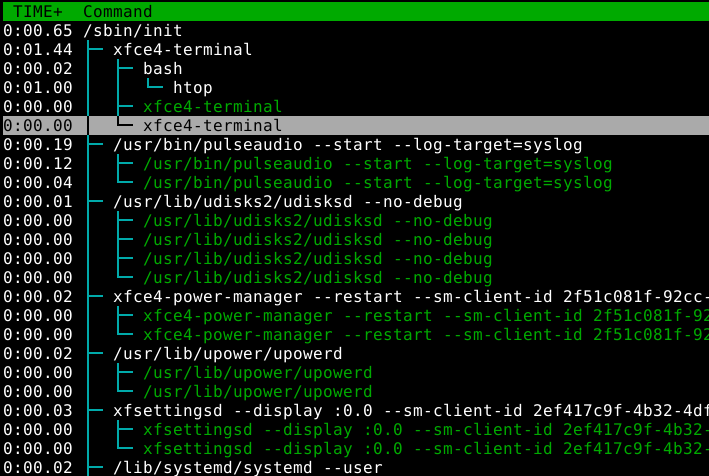
\includegraphics[width=0.9\textwidth]{img/tree}
\end{figure}

The init process is \verb|/sbin/init| and it's the one that start all the other
processes.

\end{document}